% !Mode:: "TeX:UTF-8"
\documentclass[12pt,a4paper]{article}

%%%%%%%%------------------------------------------------------------------------
%%%% 日常所用宏包

%% 控制页边距
% 如果是beamer文档类, 则不用geometry
\makeatletter
\@ifclassloaded{beamer}{}{\usepackage[top=2.5cm, bottom=2.5cm, left=2.5cm, right=2.5cm]{geometry}}
\makeatother

%% 控制项目列表
\usepackage{enumerate}

%% 多栏显示
\usepackage{multicol}

%% 算法环境
\usepackage{algorithm}  
\usepackage{algorithmic} 
\usepackage{float} 

%% 网址引用
\usepackage{url}

%% 控制矩阵行距
\renewcommand\arraystretch{1.4}

%% hyperref宏包,生成可定位点击的超链接,并且会生成pdf书签
\makeatletter
\@ifclassloaded{beamer}{
\usepackage{hyperref}
\usepackage{ragged2e} % 对齐
}{
\usepackage[%
    pdfstartview=FitH,%
    CJKbookmarks=true,%
    bookmarks=true,%
    bookmarksnumbered=true,%
    bookmarksopen=true,%
    colorlinks=true,%
    citecolor=blue,%
    linkcolor=blue,%
    anchorcolor=green,%
    urlcolor=blue%
]{hyperref}
}
\makeatother



\makeatletter % 如果是 beamer 不需要下面两个包
\@ifclassloaded{beamer}{
\mode<presentation>
{
} 
}{
%% 控制标题
\usepackage{titlesec}
%% 控制目录
\usepackage{titletoc}
}
\makeatother

%% 控制表格样式
\usepackage{booktabs}

%% 控制字体大小
\usepackage{type1cm}

%% 首行缩进,用\noindent取消某段缩进
\usepackage{indentfirst}

%% 支持彩色文本、底色、文本框等
\usepackage{color,xcolor}

%% AMS LaTeX宏包: http://zzg34b.w3.c361.com/package/maths.htm#amssymb
\usepackage{amsmath,amssymb}
%% 多个图形并排
\usepackage{subfig}
%%%% 基本插图方法
%% 图形宏包
\usepackage{graphicx}
\newcommand{\red}[1]{\textcolor{red}{#1}}
\newcommand{\blue}[1]{\structure{#1}}
\newcommand{\brown}[1]{\textcolor{brown}{#1}}
\newcommand{\green}[1]{\textcolor{green}{#1}}


%%%% 基本插图方法结束

%%%% pgf/tikz绘图宏包设置
\usepackage{pgf,tikz}
\usetikzlibrary{shapes,automata,snakes,backgrounds,arrows}
\usetikzlibrary{mindmap}
%% 可以直接在latex文档中使用graphviz/dot语言,
%% 也可以用dot2tex工具将dot文件转换成tex文件再include进来
%% \usepackage[shell,pgf,outputdir={docgraphs/}]{dot2texi}
%%%% pgf/tikz设置结束


\makeatletter % 如果是 beamer 不需要下面两个包
\@ifclassloaded{beamer}{

}{
%%%% fancyhdr设置页眉页脚
%% 页眉页脚宏包
\usepackage{fancyhdr}
%% 页眉页脚风格
\pagestyle{plain}
}

%% 有时会出现\headheight too small的warning
\setlength{\headheight}{15pt}

%% 清空当前页眉页脚的默认设置
%\fancyhf{}
%%%% fancyhdr设置结束


\makeatletter % 对 beamer 要重新设置
\@ifclassloaded{beamer}{

}{
%%%% 设置listings宏包用来粘贴源代码
%% 方便粘贴源代码,部分代码高亮功能
\usepackage{listings}

%% 设置listings宏包的一些全局样式
%% 参考http://hi.baidu.com/shawpinlee/blog/item/9ec431cbae28e41cbe09e6e4.html
\lstset{
showstringspaces=false,              %% 设定是否显示代码之间的空格符号
numbers=left,                        %% 在左边显示行号
numberstyle=\tiny,                   %% 设定行号字体的大小
basicstyle=\footnotesize,                    %% 设定字体大小\tiny, \small, \Large等等
keywordstyle=\color{blue!70}, commentstyle=\color{red!50!green!50!blue!50},
                                     %% 关键字高亮
frame=shadowbox,                     %% 给代码加框
rulesepcolor=\color{red!20!green!20!blue!20},
escapechar=`,                        %% 中文逃逸字符,用于中英混排
xleftmargin=2em,xrightmargin=2em, aboveskip=1em,
breaklines,                          %% 这条命令可以让LaTeX自动将长的代码行换行排版
extendedchars=false                  %% 这一条命令可以解决代码跨页时,章节标题,页眉等汉字不显示的问题
}}
\makeatother
%%%% listings宏包设置结束


%%%% 附录设置
\makeatletter % 对 beamer 要重新设置
\@ifclassloaded{beamer}{

}{
\usepackage[title,titletoc,header]{appendix}
}
\makeatother
%%%% 附录设置结束


%%%% 日常宏包设置结束
%%%%%%%%------------------------------------------------------------------------


%%%%%%%%------------------------------------------------------------------------
%%%% 英文字体设置结束
%% 这里可以加入自己的英文字体设置
%%%%%%%%------------------------------------------------------------------------

%%%%%%%%------------------------------------------------------------------------
%%%% 设置常用字体字号,与MS Word相对应

%% 一号, 1.4倍行距
\newcommand{\yihao}{\fontsize{26pt}{36pt}\selectfont}
%% 二号, 1.25倍行距
\newcommand{\erhao}{\fontsize{22pt}{28pt}\selectfont}
%% 小二, 单倍行距
\newcommand{\xiaoer}{\fontsize{18pt}{18pt}\selectfont}
%% 三号, 1.5倍行距
\newcommand{\sanhao}{\fontsize{16pt}{24pt}\selectfont}
%% 小三, 1.5倍行距
\newcommand{\xiaosan}{\fontsize{15pt}{22pt}\selectfont}
%% 四号, 1.5倍行距
\newcommand{\sihao}{\fontsize{14pt}{21pt}\selectfont}
%% 半四, 1.5倍行距
\newcommand{\bansi}{\fontsize{13pt}{19.5pt}\selectfont}
%% 小四, 1.5倍行距
\newcommand{\xiaosi}{\fontsize{12pt}{18pt}\selectfont}
%% 大五, 单倍行距
\newcommand{\dawu}{\fontsize{11pt}{11pt}\selectfont}
%% 五号, 单倍行距
\newcommand{\wuhao}{\fontsize{10.5pt}{10.5pt}\selectfont}
%%%%%%%%------------------------------------------------------------------------


%% 设定段间距
\setlength{\parskip}{0.5\baselineskip}

%% 设定行距
\linespread{1}


%% 设定正文字体大小
% \renewcommand{\normalsize}{\sihao}

%制作水印
\RequirePackage{draftcopy}
\draftcopyName{XTUMESH}{100}
\draftcopySetGrey{0.90}
\draftcopyPageTransform{40 rotate}
\draftcopyPageX{350}
\draftcopyPageY{80}

%%%% 个性设置结束
%%%%%%%%------------------------------------------------------------------------


%%%%%%%%------------------------------------------------------------------------
%%%% bibtex设置

%% 设定参考文献显示风格
% 下面是几种常见的样式
% * plain: 按字母的顺序排列,比较次序为作者、年度和标题
% * unsrt: 样式同plain,只是按照引用的先后排序
% * alpha: 用作者名首字母+年份后两位作标号,以字母顺序排序
% * abbrv: 类似plain,将月份全拼改为缩写,更显紧凑
% * apalike: 美国心理学学会期刊样式, 引用样式 [Tailper and Zang, 2006]

\makeatletter
\@ifclassloaded{beamer}{
\bibliographystyle{apalike}
}{
\bibliographystyle{unsrt}
}
\makeatother


%%%% bibtex设置结束
%%%%%%%%------------------------------------------------------------------------

%%%%%%%%------------------------------------------------------------------------
%%%% xeCJK相关宏包

\usepackage{xltxtra,fontspec,xunicode}
\usepackage[slantfont, boldfont]{xeCJK} 

%% 针对中文进行断行
\XeTeXlinebreaklocale "zh"             

%% 给予TeX断行一定自由度
\XeTeXlinebreakskip = 0pt plus 1pt minus 0.1pt

%%%% xeCJK设置结束                                       
%%%%%%%%------------------------------------------------------------------------

%%%%%%%%------------------------------------------------------------------------
%%%% xeCJK字体设置

%% 设置中文标点样式,支持quanjiao、banjiao、kaiming等多种方式
\punctstyle{kaiming}                                        
                                                     
%% 设置缺省中文字体
\setCJKmainfont[BoldFont={Adobe Heiti Std}, ItalicFont={Adobe Kaiti Std}]{Adobe Song Std}   
%% 设置中文无衬线字体
\setCJKsansfont[BoldFont={Adobe Heiti Std}]{Adobe Kaiti Std}  
%% 设置等宽字体
\setCJKmonofont{Adobe Heiti Std}                            

%% 英文衬线字体
\setmainfont{DejaVu Serif}                                  
%% 英文等宽字体
\setmonofont{DejaVu Sans Mono}                              
%% 英文无衬线字体
\setsansfont{DejaVu Sans}                                   

%% 定义新字体
\setCJKfamilyfont{song}{Adobe Song Std}                     
\setCJKfamilyfont{kai}{Adobe Kaiti Std}
\setCJKfamilyfont{hei}{Adobe Heiti Std}
\setCJKfamilyfont{fangsong}{Adobe Fangsong Std}
\setCJKfamilyfont{lisu}{LiSu}
\setCJKfamilyfont{youyuan}{YouYuan}

%% 自定义宋体
\newcommand{\song}{\CJKfamily{song}}                       
%% 自定义楷体
\newcommand{\kai}{\CJKfamily{kai}}                         
%% 自定义黑体
\newcommand{\hei}{\CJKfamily{hei}}                         
%% 自定义仿宋体
\newcommand{\fangsong}{\CJKfamily{fangsong}}               
%% 自定义隶书
\newcommand{\lisu}{\CJKfamily{lisu}}                       
%% 自定义幼圆
\newcommand{\youyuan}{\CJKfamily{youyuan}}                 

%%%% xeCJK字体设置结束
%%%%%%%%------------------------------------------------------------------------

%%%%%%%%------------------------------------------------------------------------
%%%% 一些关于中文文档的重定义
\newcommand{\chntoday}{\number\year\,年\,\number\month\,月\,\number\day\,日}
%% 数学公式定理的重定义

%% 中文破折号,据说来自清华模板
\newcommand{\pozhehao}{\kern0.3ex\rule[0.8ex]{2em}{0.1ex}\kern0.3ex}

\newtheorem{example}{例}                                   
\newtheorem{theorem}{定理}[section]                         
\newtheorem{definition}{定义}
\newtheorem{axiom}{公理}
\newtheorem{property}{性质}
\newtheorem{proposition}{命题}
\newtheorem{lemma}{引理}
\newtheorem{corollary}{推论}
\newtheorem{remark}{注解}
\newtheorem{condition}{条件}
\newtheorem{conclusion}{结论}
\newtheorem{assumption}{假设}

\makeatletter %
\@ifclassloaded{beamer}{

}{
%% 章节等名称重定义
\renewcommand{\contentsname}{目录}     
\renewcommand{\indexname}{索引}
\renewcommand{\listfigurename}{插图目录}
\renewcommand{\listtablename}{表格目录}
\renewcommand{\appendixname}{附录}
\renewcommand{\appendixpagename}{附录}
\renewcommand{\appendixtocname}{附录}
%% 设置chapter、section与subsection的格式
\titleformat{\chapter}{\centering\huge}{第\thechapter{}章}{1em}{\textbf}
\titleformat{\section}{\centering\sihao}{\thesection}{1em}{\textbf}
\titleformat{\subsection}{\xiaosi}{\thesubsection}{1em}{\textbf}
\titleformat{\subsubsection}{\xiaosi}{\thesubsubsection}{1em}{\textbf}

\@ifclassloaded{book}{

}{
\renewcommand{\abstractname}{摘要}
}
}
\makeatother

\renewcommand{\figurename}{图}
\renewcommand{\tablename}{表}

\makeatletter
\@ifclassloaded{book}{
\renewcommand{\bibname}{参考文献}
}{
\renewcommand{\refname}{参考文献} 
}
\makeatother

\floatname{algorithm}{算法}
\renewcommand{\algorithmicrequire}{\textbf{输入:}}
\renewcommand{\algorithmicensure}{\textbf{输出:}}

%%%% 中文重定义结束
%%%%%%%%------------------------------------------------------------------------


\title{线性弹性模型}
%\author{}
\date{\chntoday}

\begin{document}
\maketitle

\section{应力}

作用于物体的外力通常可以分为两类,即面力和体力。面力是指分布在物体表面上的外力,不一定作用在物体表面的每一个质点上,比如压力。体力是指分布在物体体积内的外力,即作用在弹性体内每一个质点上,比如重力。

物体由于外因(受力、湿度、温度场变化等)而变形时,在物体内各部分之间产生相互作用的内力,以抵抗这种
外因的作用,并试图使物体从变形后的位置恢复到变形前的位置。

\begin{figure}[H]
\centering

\includegraphics[scale=0.4]{./figures/1.png}
\caption{}
\end{figure}

应力:在所考察的截面某一点单位面积上的内力称为应力。物体内的一点有无数个截面,这里选取一个截面,考虑该截面上的应力。弹性体受外力以后,其内部将产生应力。
应力是矢量,沿外法线方向的应力分量称为正应力或法向应力,同截面相切的应力分量称为剪应力或切应力。下图中的 $\sigma _N$ 为正应力,$\tau _N$ 为剪应力。

\begin{figure}[H]
\centering
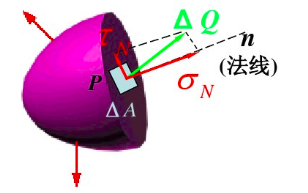
\includegraphics[scale=0.5]{./figures/2.png}
\caption{}
\end{figure}

物体中一点在所有截面上的应力称为该点的应力状态,即通过一点的所有单位面积的内力的集合。
虽然过一点可作无数个平面,但不需要用无数个平面上的应力来描述该点的应力状态,只需用过一点的任意一组相互垂直的三个平面上的应力就可代表该点的应力状态,而其它截面上的应力都可用这组应力与截面的方位关系来表示。

为了表示某一点 $P$ 点的应力状态,引入微分单元体(又称为应力单元,边长分别为 $dx,dy,dz$),约定微分单元体相对面上的应力等值、反向、共线。

\begin{figure}[H]
\centering
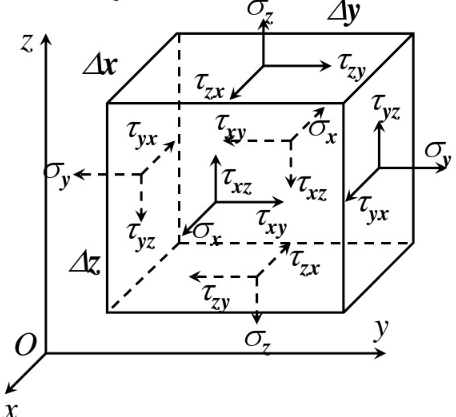
\includegraphics[scale=0.5]{./figures/17.png}
\caption{}
\end{figure}

在坐标系中以 $P$ 点为端点,取与坐标轴平行的平面组成六面体,选取六面体上三个相互垂直的平面,用这三个平面上的应力来描述 $P$ 点的应力状态。

将每一面上的应力分解为一个正应力和两个剪应力,分别与三个坐标轴平行。

正应力用 $\sigma$ 表示,为了表面这个正应力的作用面和作用方向,加上一个下标,例如:正应力 $\sigma_x$ 是作用在垂直于 $x$ 轴的面上,同时也是沿着 $x$ 轴的方向作用的。

剪应力用 $\tau$ 来表示,并加上两个下标,前一个下标表明作用面垂直于哪一个坐标轴,后一个下标表明作用方向沿着哪一个坐标轴。例如:剪应力 $\tau_{xy}$ 是作用在垂直于 $x$ 轴的面上,并且沿着 $y$ 轴的方向作用的。

综上,应力分量的第一个下标表示作用面,第二个下标表示作用方向。正应力的两个下标是一样的,故用一个下标简写。

\begin{figure}[H]
\centering
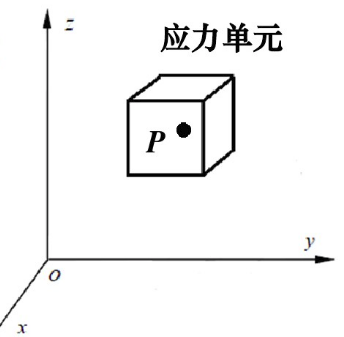
\includegraphics[scale=0.4]{./figures/3.png}
\caption{}
\end{figure}

\begin{figure}[H]
\centering
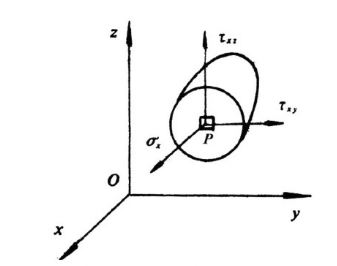
\includegraphics[scale=0.5]{./figures/4.png}
\caption{}
\end{figure}

\begin{figure}[H]
\centering
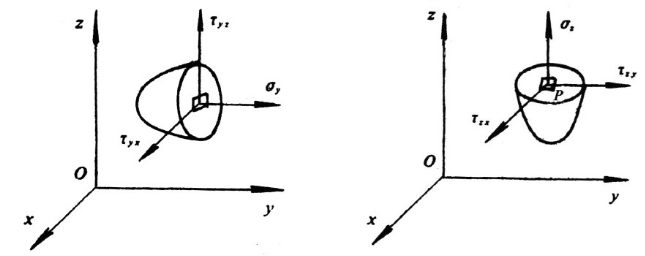
\includegraphics[scale=0.5]{./figures/5.png}
\caption{}
\end{figure}

为判断应力分量的正负号,这里规定:

正面:外法线方向与坐标轴正方向一致;

负面:外法线方向与坐标轴正方向相反;

正面上:应力方向与坐标轴正方向一致时为正;

负面上:应力方向与坐标轴正方向相反时为正;

\begin{figure}[H]
\centering
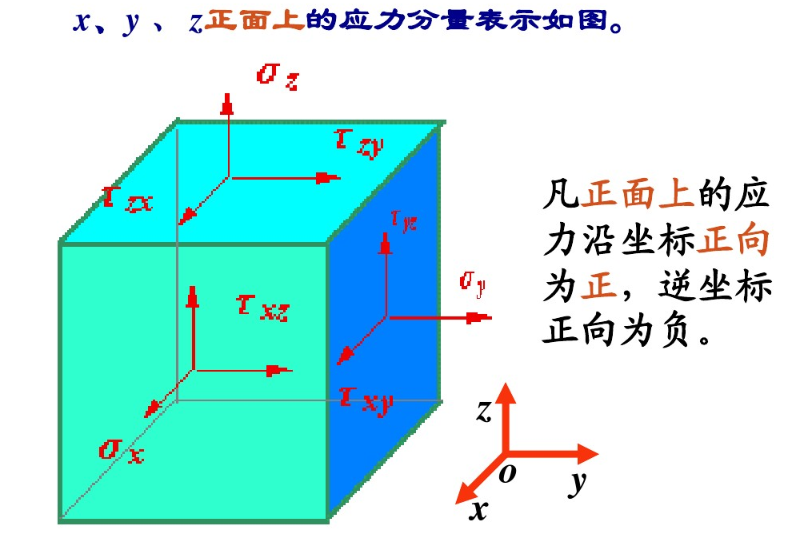
\includegraphics[scale=0.5]{./figures/18.png}
\caption{}
\end{figure}

如果某一个面上的外法线是沿着坐标轴的正方向,这个面上的应力就以沿坐标轴正方向为正,沿坐标轴负方向为负。

相反,如果某一个面上的外法线是沿着坐标轴的负方向,这个面上的应力就以沿坐标轴负方向为正,沿坐标轴正方向为负。

\begin{figure}[H]
\centering

\includegraphics[scale=0.5]{./figures/6.png}
\caption{}
\end{figure}

三个正面上共有九个应力分量(包括三个正应力和六个切应力)。此九个应力分量可写成如下矩阵形式
$$
\begin{bmatrix}
\sigma _x & \tau_{xy} & \tau_{xz} \\
\tau_{yx} & \sigma _y & \tau_{yz} \\
\tau_{zx} & \tau_{zy} & \sigma _z
\end{bmatrix}
$$

张量中,$x \to x_1 , y \to x_2 , z \to x_3$
$$
\sigma _{ij} =
\begin{bmatrix}
\sigma _x & \tau_{xy} & \tau_{xz} \\
\tau_{yx} & \sigma _y & \tau_{yz} \\
\tau_{zx} & \tau_{zy} & \sigma _z
\end{bmatrix}=
\begin{bmatrix}
\sigma _{11} & \sigma_{12} & \sigma_{13} \\
\sigma_{21} & \sigma _{22} & \sigma_{23} \\
\sigma_{31} & \sigma_{32} & \sigma_{33}
\end{bmatrix}
$$

切应力互等定理:作用在相互垂直的两截面上的切应力大小相等。

由于切应力互等定理,上列矩阵中对角的切应力是相等的,即:$\tau_{xy}=\tau_{yx}, \tau_{yz}=\tau_{zy}, \tau_{xz}=\tau_{zx}$,因此,这个矩阵为对称矩阵,并且九个应力分量中只有六个应力分量是独立的。即应力张量是一个对称的二阶张量。

一般来说,弹性体内各点的应力状态都不相同,因此,描述弹性体内应力状态的上述六个应力分量并不是常量,而是 $x,y,z$ 的函数。

已知一点的应力状态,可以求得经过该点的任何截面上的应力。

过 $M$ 点用与坐标平面平行的三个平面截取一微分单元体,在过此单元作一个与 $M$ 点相距为无穷小的任意斜截面。截面 $ABC$ 和过 $M$ 点的单元体平面形成一个微分四面体。知道 $M$ 点的应力状态,以及截面 $ABC$ 与各坐标平面的方向关系,就可求得截面 $ABC$ 上的应力。并且截面 $ABC$ 上的应力可以认为是过 $M$ 点任意截面上的应力。即当截面 $ABC$ 趋近于 $M$ 点时,截面 $ABC$ 上的应力就趋近于经过 $M$ 点的任一斜面上的应力。

\begin{figure}[H]
\centering
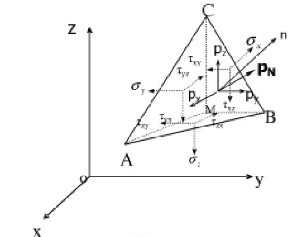
\includegraphics[scale=0.5]{./figures/7.png}
\caption{}
\end{figure}

截面 $ABC$ 外法线向量与各坐标轴正向夹角的方向余弦分别记为 $l,m,n$.

\begin{figure}[H]
\centering
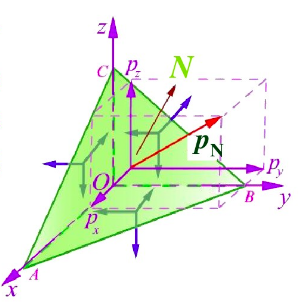
\includegraphics[scale=0.5]{./figures/8.png}
\caption{}
\end{figure}

$\triangle ABC$ 的面积为 $dS$,根据平面图形面积投影定理,$\triangle OBC$ 的面积为 $mdS$,$\triangle OAB$ 的面积为 $ndS$,$\triangle OAC$ 的面积为 $ldS$,
$$
\overrightarrow{p_N}=p_x \overrightarrow{i} +p_y \overrightarrow{j} +p_z \overrightarrow{k}
$$
由$x$轴平衡条件得到
$$
p_x dS-\sigma_x l dS-\tau_{yx}mdS-\tau_{zx}ndS=0
$$
即
$$
p_x -\sigma_x l -\tau_{yx}m-\tau_{zx}n=0
$$
$$
p_x =\sigma_x l +\tau_{yx}m+\tau_{zx}n
$$
同理可得
$$
p_y =\tau_{xy} l +\sigma_x m +\tau_{zy}n
$$
$$
p_z =\tau_{xz} l +\tau_{yz}m + \sigma_z n
$$
写成矩阵形式:
$$
\begin{bmatrix}
p_x \\
p_y \\
p_z
\end{bmatrix}=
\begin{bmatrix}
\sigma _x & \tau_{yx} & \tau_{zx} \\
\tau_{xy} & \sigma _y & \tau_{zy} \\
\tau_{xz} & \tau_{yz} & \sigma _z
\end{bmatrix}
\begin{bmatrix}
l \\
m \\
n
\end{bmatrix}
$$
上式即是平面 $ABC$ 上的应力。

因此,已知应力张量,可以确定任意截面上的应力,当然也就可以确定这个截面上的正应力 $\overrightarrow{\sigma _N}$ 和切应力 $\overrightarrow{\tau_N}$

将 $\overrightarrow{p_N}$ 的各分量向 $\overrightarrow{N}$ 方向投影:
$$
\overrightarrow{\sigma _N}=l\cdot p_x + m\cdot p_y + n\cdot p_z=
\begin{bmatrix}
l & m & n\\
\end{bmatrix}
\begin{bmatrix}
p_x \\
p_y \\
p_z
\end{bmatrix}=
\begin{bmatrix}
l & m & n\\
\end{bmatrix}\sigma _{ij}^T
\begin{bmatrix}
l \\
m \\
n
\end{bmatrix}
$$
切应力:
$$
\overrightarrow{\tau_N}=\sqrt{|\overrightarrow{p_N}|^2-|\overrightarrow{\sigma _N}|^2}
$$

\begin{figure}[H]
\centering
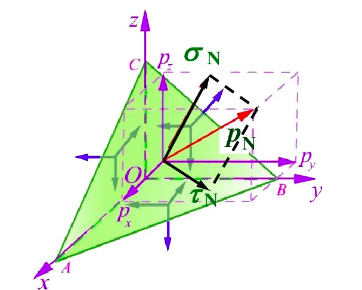
\includegraphics[scale=0.5]{./figures/9.png}
\caption{}
\end{figure}

因此,已知物体内任一点的应力状态,可以求出经过该点的任意斜面上的正应力和切应力。

如果作用在某一截面上的全应力和这一截面垂直,即该截面上只有正应力,切应力为零,则这一截面称为主平面,其法线方向称为应力主方向或应力主轴,其上的应力称为主应力。即 $\overrightarrow{\tau_N}=0$.

\section{应变}
由于外部因素作用(温度改变等)引起物体内部各质点位置的改变称为位移。物体内任意一点的位移,可以用它 在$x,y,z$三个坐标轴上的投影 $u,v,w$ 来表示,这三个投影称为该点的位移分量。一般来说,位移分量也是 $x,y,z$ 的函数。

位移类别:

刚体位移:位移内部各点位置变化,但仍保持初始状态相对位置不变(即物体内任意两点之间距离保持不变)

刚体位移包括平移,转动。

\begin{figure}[H]
\centering
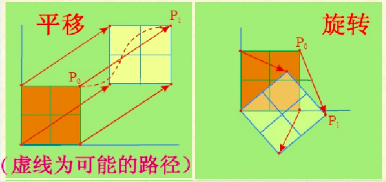
\includegraphics[scale=0.5]{./figures/10.png}
\caption{}
\end{figure}

变形位移:位移不仅使得位置改变,而且改变了物体内部各个点的相对位置,即物体的形状发生改变。

变形位移包括形状改变和体积改变。

\begin{figure}[H]
\centering
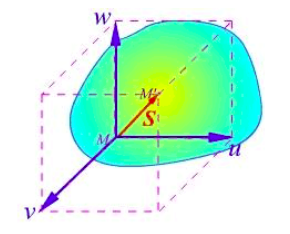
\includegraphics[scale=0.5]{./figures/11.png}
\caption{}
\end{figure}

一个物体受作用力后,其内部质点不仅要发生相对位置的改变(产生了位移),而且要产生形状的变化(产生了变形),物体的变形程度用应变来度量,即应变是表示变形大小的一个物理量。物体变形时,其体内各质点在各方向上都会有应变。应变与位移有密切的联系,位移一旦确定,那么应变也就确定了。

因此,弹性体在受外力以后,将发生位移和变形。

应变与所考虑的点的位置和所选取的方向有关。物体中一点在所有可能方向上的应变的全体称为该点的应变状态。它由通过该点的线段长度的所有变化的总体,以及由该点放射出的任何两条射线之间夹角的所有变化的总体构成。

为了描述弹性体内任一点 $P$ 的应变状态,在这一点沿着坐标轴的正方向取三个微小线段,弹性体变形以后,这三个线段的长度以及它们之间的直角都将改变。线段的每单位长度的伸缩称为正应变,线段之间直角的改变称为剪应变。

正应变用 $\varepsilon$ 表示,$\varepsilon_x$ 表示 $x$ 方向的线段的正应变,其余类推。正应变以伸长时为正,缩短时为负。

剪应变用 $\gamma$ 表示,$\gamma_{xy}$ 表示 $x$ 与 $y$ 两方向的线段之间的直角的改变,其余类推。剪应变以直角变小时为正,变大时为负。

正应变又叫线应变,它是某一方向上微小线段因变形产生的长度增量(伸长时为正)与原长度的比值。

剪应变又叫角应变或切应变,它是两个相互垂直方向上的微小线段在变形后夹角的改变量(以弧度表示,角度减小时为正)。

此外,还有一种应变,叫做体应变,定义为单位体积的改变量,一般用 $\theta$ 表示。当体积 $V$ 增大或者缩小时 $\Delta V$ 时,体应变$\theta=\Delta V/V$,无限小应变条件下,
$$
\theta=\varepsilon_x+\varepsilon_y+\varepsilon_z
$$
体应变是由线应变和切应变引起的,并且由上式可知,在无限小应变条件下,体应变只与线应变有关,与切应变无关。

设单元体的初始边长为 $dx,dy,dz$,变形前的体积为 $V_0=dxdydz$,切应变引起的体积变化是高阶微量,可以忽略,则体积的变化只是由线应变引起的。$x$ 方向上的线应变为 $\varepsilon_x=\frac{r_x-dx}{dx}$,所以 $r_x=dx(1+\varepsilon_x)$.同理,$r_y=dy(1+\varepsilon_y),r_z=dz(1+\varepsilon_z)$.变形后的单元体的体积为
$$
V_1=r_xr_yr_z=dxdydz(1+\varepsilon_x)(1+\varepsilon_y)(1+\varepsilon_z)
$$
略去二阶及以上的高阶微量,得到单元体单位体积的变化(单位体积变化率)
$$
\theta=(V_1-V_0)/V_0=\varepsilon_x+\varepsilon_y+\varepsilon_z
$$

可以证明一旦已知通过一点并且平行一组相互垂直坐标轴的三条线段的长度和角度的变化,就能计算出通过该点的任一微小线段的正应变,以及经过该点的任意两个微小线段之间的夹角的变化。

与应力分析一样,点的应变状态也是二阶对称张量。它可由一点在三个正交的坐标($x_1,x_2,x_3$)方向的应变分量 $\varepsilon_{ij},(i,j=1,2,3)$ 来确定,其中 $\varepsilon_{11},\varepsilon_{22},\varepsilon_{33}$ 分别为 $x_1,x_2,x_3$ 方向的正应变,而 $\varepsilon_{12}$ 反映 $x_1,x_2$ 两方向上微小线段的夹角改变量(事实上,$\varepsilon_{12}$ 为 $x_1,x_2$ 方向微线段间夹角改变量的一半),其余类推。在九个应变分量 $\varepsilon_{ij}$ 中,$\varepsilon_{ij}=\varepsilon_{ji}$,即只有六个独立分量,它们称为在该点的应变分量。一般来说,应变分量也是 $x,y,z$ 的函数。

把这九个应变分量写成矩阵形式
$$
\varepsilon_{ij}=
\begin{bmatrix}
\varepsilon_{11} & \varepsilon_{12} & \varepsilon_{13} \\
\varepsilon_{21} & \varepsilon_{22} & \varepsilon_{23} \\
\varepsilon_{31} & \varepsilon_{32} & \varepsilon_{33}
\end{bmatrix}=
\begin{bmatrix}
\varepsilon_{x} & \frac{1}{2}\gamma_{xy} & \frac{1}{2}\gamma_{xz} \\
\frac{1}{2}\gamma_{xy} & \varepsilon_{y} & \frac{1}{2}\gamma_{yz} \\
\frac{1}{2}\gamma_{xz} & \frac{1}{2}\gamma_{yz} & \varepsilon_{z}
\end{bmatrix}
$$

应变张量准确描述了物体变形后的局部的几何性质。把应变张量分解为
$$
\begin{bmatrix}
\varepsilon_{11} & \varepsilon_{12} & \varepsilon_{13} \\
\varepsilon_{21} & \varepsilon_{22} & \varepsilon_{23} \\
\varepsilon_{31} & \varepsilon_{32} & \varepsilon_{33}
\end{bmatrix}=\begin{bmatrix}
\varepsilon_{11}-\varepsilon_m & \varepsilon_{12} & \varepsilon_{13} \\
\varepsilon_{21} & \varepsilon_{22}-\varepsilon_m & \varepsilon_{23} \\
\varepsilon_{31} & \varepsilon_{32} & \varepsilon_{33}-\varepsilon_m
\end{bmatrix}+\begin{bmatrix}
\varepsilon_m & 0 & 0 \\
0 & \varepsilon_m & 0 \\
0 & 0 & \varepsilon_m
\end{bmatrix}
$$
其中,$\varepsilon_m=\frac{\varepsilon_{11}+\varepsilon_{22}+\varepsilon_{33}}{3}$ 称为平均正应变,
$\begin{bmatrix}
\varepsilon_{11}-\varepsilon_m & \varepsilon_{12} & \varepsilon_{13} \\
\varepsilon_{21} & \varepsilon_{22}-\varepsilon_m & \varepsilon_{23} \\
\varepsilon_{31} & \varepsilon_{32} & \varepsilon_{33}-\varepsilon_m
\end{bmatrix}$ 反映微元体的形状变化,
$\begin{bmatrix}
\varepsilon_m & 0 & 0 \\
0 & \varepsilon_m & 0 \\
0 & 0 & \varepsilon_m
\end{bmatrix}$ 反映微元体的体积变化。
当应变不一定是无限小时,物体的体积变化不能只是通过$\begin{bmatrix}
\varepsilon_m & 0 & 0 \\
0 & \varepsilon_m & 0 \\
0 & 0 & \varepsilon_m
\end{bmatrix}$ 来反映,因为这个时候的体积变化还与切应变有关。

考虑一个法线为 $\overrightarrow{N}$ 的斜平面,方向余弦 $(l_1=l,l_2=m,l_3=n)$,斜平面上应变 $\overrightarrow{q_N}$:
$$
\begin{bmatrix}
q_{N1} \\
q_{N2} \\
q_{N3}
\end{bmatrix}=
\begin{bmatrix}
\varepsilon_{11} & \varepsilon_{12} & \varepsilon_{13} \\
\varepsilon_{21} & \varepsilon_{22} & \varepsilon_{23} \\
\varepsilon_{31} & \varepsilon_{32} & \varepsilon_{33}
\end{bmatrix}
\begin{bmatrix}
l \\
m \\
n
\end{bmatrix}
$$
如果应变矢量 $\overrightarrow{q_N}$ 正在平面法线 $\overrightarrow{N}$ 方向上,则在这一方向上剪应变为 $0$,该法线方向即为主方向(或应变主轴),相应的应变称为主应变。

\section{几何方程}
应变分量与位移分量之间有一定的几何关系,这就是所谓的几何方程(用位移导数表示应变)。

$oxy$ 平面应变与位移的关系

起于 $P(x,y)$ 点,平行于 $x$ 轴的微元线段 $PQ$(长度$dx$)移动、转动。

\begin{figure}[H]
\centering
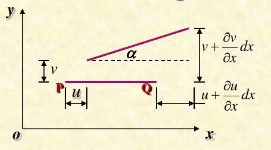
\includegraphics[scale=0.5]{./figures/13.png}
\caption{}
\end{figure}

平行于 $y$ 轴的微元线段 $PT$(长度$dy$)移动、转动。

\begin{figure}[H]
\centering
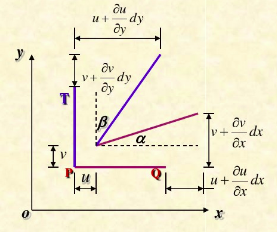
\includegraphics[scale=0.5]{./figures/14.png}
\caption{}
\end{figure}

$P(x,y)$ 点位移是:$(u,v)$,即 $P$ 点 $x$ 方向的位移为 $u(x,y)$,$y$ 方向的位移为$v(x,y)$;
$Q$ 点位移是:$(u',v')$,即 $Q$ 点 $x$ 方向的位移为 $u(x+dx,y)\approx u+\frac{\partial u}{\partial x}dx$,$y$ 方向的位移为$v(x+dx,y)\approx v+\frac{\partial v}{\partial x}dx$;
$T$ 点位移是:$(u'',v'')$,即 $T$ 点 $x$ 方向的位移为 $u(x,y+dy)\approx u+\frac{\partial u}{\partial y}dy$,$y$ 方向的位移为 $v(x,y+dy)\approx v+\frac{\partial v}{\partial y}dy$;
即 $Q$ 点位移为 $(u+\frac{\partial u}{\partial x}dx,v+\frac{\partial v}{\partial x}dx)$,$T$ 点位移为 $(u+\frac{\partial u}{\partial y}dy,v+\frac{\partial v}{\partial y}dy)$

因此,$PQ$ 在 $x$ 方向的正应变:
$$
\varepsilon_x=\frac{(u+\frac{\partial u}{\partial x}dx)-u}{dx}=\frac{\partial u}{\partial x}
$$
转角 $\alpha$:
$$
\alpha=\frac{(v+\frac{\partial v}{\partial x}dx)-v}{dx}=\frac{\partial v}{\partial x}
$$
$PT$ 在 $y$ 方向的正应变:
$$
\varepsilon_y=\frac{(v+\frac{\partial v}{\partial y}dx)-v}{dy}=\frac{\partial v}{\partial y}
$$
转角 $\beta$:
$$
\beta=\frac{(u+\frac{\partial u}{\partial y}dy)-u}{dy}=\frac{\partial u}{\partial y}
$$
因此,正应变为:
$$
\varepsilon_x=\frac{\partial u}{\partial x},\varepsilon_y=\frac{\partial v}{\partial y}
$$
$P$ 点两直角线段夹角的变化,即剪应变为:
$$
\gamma_{xy}=\alpha +\beta =\frac{\partial v}{\partial x}+\frac{\partial u}{\partial y}
$$
其他平面,结果类似。

$oyz$ 平面:
$$
\varepsilon_z=\frac{\partial w}{\partial z},\gamma_{yz}=\frac{\partial v}{\partial z}+\frac{\partial w}{\partial y}
$$

$ozx$平面:
$$
\gamma_{zx}=\frac{\partial w}{\partial x}+\frac{\partial u}{\partial z}
$$

最后结果:
$$
\varepsilon_x=\frac{\partial u}{\partial x},\gamma_{xy}=\frac{\partial u}{\partial y}+\frac{\partial v}{\partial x}
$$
$$
\varepsilon_y=\frac{\partial v}{\partial y},\gamma_{yz}=\frac{\partial v}{\partial z}+\frac{\partial w}{\partial y}
$$
$$
\varepsilon_z=\frac{\partial w}{\partial z},\gamma_{zx}=\frac{\partial w}{\partial x}+\frac{\partial u}{\partial z}
$$

上式表明了一点处的位移分量和应变分量所应满足的关系,称为几何方程,也称为柯西关系。

矩阵表示:
$$
\varepsilon_{ij}=
\begin{bmatrix}
\varepsilon_{11} & \varepsilon_{12} & \varepsilon_{13} \\
\varepsilon_{21} & \varepsilon_{22} & \varepsilon_{23} \\
\varepsilon_{31} & \varepsilon_{32} & \varepsilon_{33}
\end{bmatrix}=
\begin{bmatrix}
\varepsilon_{x} & \frac{1}{2}\gamma_{xy} & \frac{1}{2}\gamma_{xz} \\
\frac{1}{2}\gamma_{xy} & \varepsilon_{y} & \frac{1}{2}\gamma_{yz} \\
\frac{1}{2}\gamma_{xz} & \frac{1}{2}\gamma_{yz} & \varepsilon_{z}
\end{bmatrix}
$$
$$
\varepsilon_{ij}=
\begin{bmatrix}
\frac{\partial u}{\partial x} & \frac{1}{2}(\frac{\partial v}{\partial x}+\frac{\partial u}{\partial y}) & \frac{1}{2}(\frac{\partial w}{\partial x}+\frac{\partial u}{\partial z}) \\
\frac{1}{2}(\frac{\partial v}{\partial x}+\frac{\partial u}{\partial y}) & \frac{\partial v}{\partial y} & \frac{1}{2}(\frac{\partial w}{\partial y}+\frac{\partial v}{\partial z}) \\
\frac{1}{2}(\frac{\partial w}{\partial x}+\frac{\partial u}{\partial z}) & \frac{1}{2}(\frac{\partial w}{\partial y}+\frac{\partial v}{\partial z}) & \frac{\partial w}{\partial z}
\end{bmatrix}
$$
$\textbf{u}=(u(x,y,z),v(x,y,z),w(x,y,z))$,那么
$$
\nabla\textbf{u}=\begin{bmatrix}
u_x & u_y & u_z \\
v_x & v_y & v_z \\
w_x & w_y & w_z 
\end{bmatrix},
\nabla\textbf{u}^T=\begin{bmatrix}
u_x & v_x & w_x \\
u_y & v_y & w_y \\
u_z & v_z & w_z 
\end{bmatrix}
$$
因此,
$$
\varepsilon = \frac{1}{2}(\nabla\textbf{u} + \nabla\textbf{u}^T) 
=\begin{bmatrix}
u_x & \frac{v_x + u_y}{2} & \frac{w_x + u_z}{2} \\
\frac{v_x + u_y}{2} & v_y & \frac{w_y + v_z}{2} \\
\frac{w_x + u_z}{2} & \frac{w_y + v_z}{2} & w_z 
\end{bmatrix}
\rightarrow 
\begin{bmatrix}
u_x \\ w_y \\ v_z \\ \frac{w_y + v_z}{2} \\ \frac{w_x + u_z}{2} \\ \frac{v_x + u_y}{2}
\end{bmatrix}
$$

由几何方程可知,当弹性体的位移分量确定时,应变分量可以通过上式确定;反过来,当应变分量确定时,位移分量却不确定,因为这里涉及到积分,需要确定积分常数,这个可以由边界条件确定。因此,位移为 $0$ 或者常数,应变一定为 $0$;应变为 $0$,位移未必为 $0$.

几何方程表示任一点的微分线段应变与位移之间的关系,适用于弹性体内的任何点。

\section{静力平衡方程}
沿三坐标轴的正向分别取长度为 $dx$、$dy$ 和 $dz$的三条棱边,由此构成一个微长单元体。同时给这个微六面体施加一个体力 $(f_x,f_y,f_z)$,微长方体共六个面,有三个正面(“前面”,“上面”,“右面”)和三个负面(“后面”,“下面”,“左面”),每个面上有一个正应力和两个剪应力。并表示出正面上由坐标增量引起的应力增量。

设 $Q(x,y,z)$ 为“后面”上的一点,过 $Q(x,y,z)$ 点的该平面上的应力分量为: $\sigma_x=\sigma_x(x,y,z)$,$\tau_{xy}=\tau_{xy}(x,y,z)$ 和 $\tau_{xz}=\tau_{xz}(x,y,z)$,那么与该平面平行并且相距为 $dx$ 的平面上的应力分量为: $\sigma_x(x+dx,y,z)$,$\tau_{xy}(x+dx,y,z)$ 和 $\tau_{xz}(x+dx,y,z)$,将这三个应力分量作泰勒展式,并略去二次及其以上的小量,得到:
$$
\sigma_x(x+dx,y,z)\approx \sigma_x+\frac{\partial\sigma_x}{\partial x}dx,\tau_{xy}(x+dx,y,z)\approx \tau_{xy}+\frac{\partial\tau_{xy}}{\partial x}dx,\tau_{xz}(x+dx,y,z)\approx \tau_{xz}+\frac{\partial\tau_{xz}}{\partial x}dx
$$
并且这两个平面上的应力方向相反。同理可得其他四个面上的应力分量。

\begin{figure}[H]
\centering
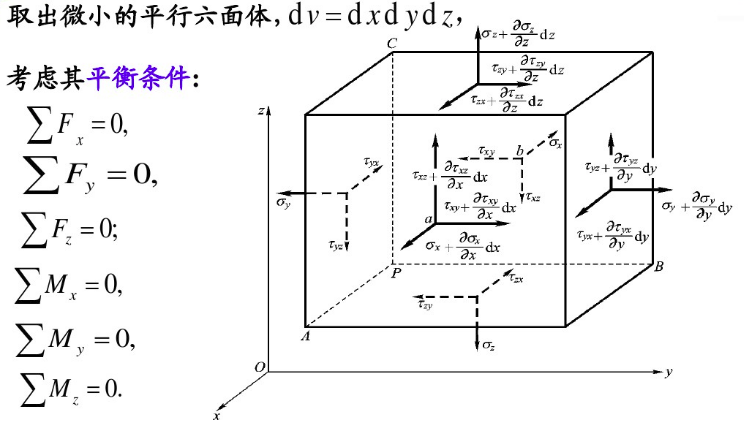
\includegraphics[scale=0.5]{./figures/15.png}
\caption{}
\end{figure}

由 $x$ 方向上力的平衡有
$$
(\sigma_x+\frac{\partial\sigma_x}{\partial x}dx)dydz-\sigma_x dydz+(\tau_{yx}+\frac{\partial\tau_{yx}}{\partial y}dy)dxdz-\tau_{yx}dxdz+(\tau_{zx}+\frac{\partial\tau_{zx}}{\partial z}dz)dxdy-\tau_{zx}dxdy+f_xdxdydz=0
$$
整理得到
$$
\frac{\partial\sigma_x}{\partial x}+\frac{\partial\tau_{yx}}{\partial y}+\frac{\partial\tau_{zx}}{\partial z}+f_x=0
$$
同理可得其他两个方向的平衡方程:
$$
\frac{\partial\tau_{xy}}{\partial x}+\frac{\partial\sigma_{y}}{\partial y}+\frac{\partial\tau_{zy}}{\partial z}+f_y=0
$$
$$
\frac{\partial\tau_{xz}}{\partial x}+\frac{\partial\tau_{yz}}{\partial y}+\frac{\partial\sigma_{x}}{\partial z}+f_z=0
$$
因此,
$$
-\nabla\cdot\begin{bmatrix}
\sigma _x & \tau_{xy} & \tau_{xz} \\
\tau_{yx} & \sigma _y & \tau_{yz} \\
\tau_{zx} & \tau_{zy} & \sigma _z
\end{bmatrix}=\begin{bmatrix}
f_x \\
f_y \\
f_z
\end{bmatrix}
$$

$$
-\nabla\cdot \sigma = \textbf{f}
$$

弹性力学考虑的是微分单元体 $dV$ 的平衡,比理论力学中考虑整体 $V$ 的平衡更加精确;因为当 $dV$ 都平衡时,能够保证 $V$ 平衡,反之不然。静力平衡方程代表了弹性体内所有点的平衡条件,并且这个平衡条件是精确的。

讨论力矩平衡时,为方便计算,将坐标原点移到微六面体的重心处。由于体力、正应力的合力都通过微六面体的重心,因此它们对三个坐标轴的力矩都为 $0$,力矩平衡方程中仅包含剪应力。

由于剪应力 $\tau_{yx}$ 和 $\tau_{zx}$ 与 $x$ 轴平行,因此对 $x$ 轴的力矩为 $0$,绕 $x$ 轴的力矩平衡方程为:
$$
\tau_{yz}dxdz\cdot\frac{1}{2}dy+(\tau_{yz}+\frac{\partial\tau_{yz}}{\partial y})dxdz\cdot\frac{1}{2}dy-\tau_{zy}dxdy\cdot\frac{1}{2}dz-(\tau_{zy}+\frac{\partial\tau_{zy}}{\partial z})dxdy\cdot\frac{1}{2}dz=0
$$
整理得:
$$
2\tau_{yz}+\frac{\partial\tau_{yz}}{\partial y}dy-2\tau_{zy}-\frac{\partial\tau_{zy}}{\partial z}dz=0
$$
略去高阶小量,得到 $\tau_{yz}=\tau_{zy}$.

同理可得对于其它两个坐标轴的力矩平衡方程:
$$
\tau_{xy}=\tau_{yx},\tau_{zx}=\tau_{xz}
$$

\section{本构方程}
各向同性材料只有两个独立的材料参数,一般材料的材料参数有五个,统称为拉梅参数,拉梅参数也称为拉梅系数或拉梅常数,用其中任意两个就可以表示其余三个参数。通常,应变-应力关系中的 $\lambda$ 和 $\mu$ 两个材料参数分别称为拉梅的第一个参数和拉梅的第二个参数。

\begin{figure}[H]
\centering
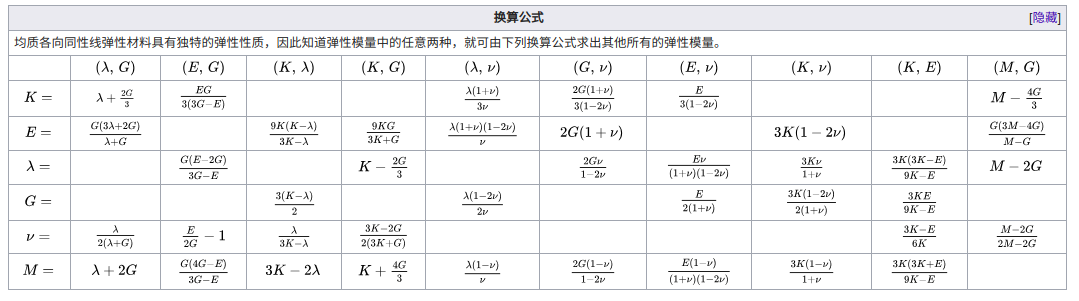
\includegraphics[scale=0.4]{./figures/19.png}
\caption{}
\end{figure}

第一参数 $\lambda$ 没有确切的物理含义,与材料的压缩性有关。在与弹性相关的环境中,$\mu$ 称为剪切模量,有时用 $G$ 表示,而不是$\mu$.通常,符号 $G$ 与使用杨氏模量配对,符号 $\lambda$ 与 $\mu$ 的使用配对。
剪切模量定义为剪应力和剪应变之比:
$$
\mu \text{ or } G = \frac{\tau}{\gamma}
$$ 
它表式材料抵抗切应变的能力。

弹性模量可视为衡量材料产生弹性变形难易程度的指标,其值越大,使材料发生一定弹性变形的应力也越大,即
材料刚度越大,亦即在一定应力作用下,发生弹性变形越小。弹性模量是描述物质弹性的物理量,是一个总称,包括“杨氏模量”、“剪切模量”、“体积模量”等。

杨氏模量是描述固体材料抵抗形变能力的物理量,是弹性模量中最常见的一种。杨氏模量衡量的是一个各向同性弹性体的刚度,它是沿纵向的弹性模量, 定义为正应力和正应变之间的比值。
$$
E = \frac{\sigma}{\epsilon}
$$
杨氏模量是表征材料性质的一
个物理量,仅取决于材料本身的物理性质。杨氏模量的大小标志了材料的刚性,杨氏模量越大,越不容易发生形
变。

泊松比 $\nu$ 是指材料在单向受拉或受压时,横向正应变与轴向正应变的绝对值的比值,也叫横向变形系数,它是反映
材料横向变形的弹性常数。比如,一根杆被拉伸时,其轴向伸长伴随着横向收缩(反之亦然)。在弹性限度内,横向应变 $\varepsilon_x$ 与轴向应变 $\varepsilon_y$ 之间存在下列关系:
$$
\varepsilon_x=-\nu\varepsilon_y
$$

剪切模量、杨氏模量与泊松比之间的关系:
$$
\lambda = \frac{\nu E}{(1 + \nu)(1 - 2\nu)},\quad \mu \text{ or } G= \frac{E}{2(1 + \nu)}
$$

本构关系: 反映物质宏观性质的数学模型,比如反映力学性质的广义胡克定理。对于不同的物质,在不同的变形条件下有不同的本构关系,也称为不同的本构模型。以下讨论的本构方程都指的是力学中的广义虎克定理(表示微分单元体上应力和应变之间的物理关系)。

\begin{figure}[H]
\centering
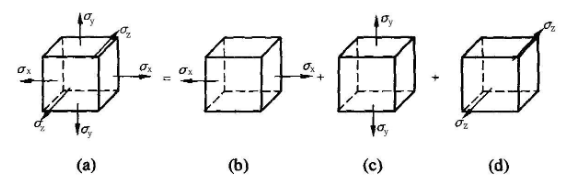
\includegraphics[scale=0.5]{./figures/16.png}
\caption{}
\end{figure}

如果 $x$ 方向受到简单拉伸(没有切应力),由杨氏模量的定义有:
$$
\sigma_x=E\varepsilon_{xx}
$$
因此,当正应力 $\sigma_x$ 单独作用时(图 $(b)$ ),微分单元体在 $x$ 方向上的线应变为 $\varepsilon_{xx}=\frac{\sigma_x}{E}$.

再由泊松比的定义有:
$$
\varepsilon_{xy}=-\nu\varepsilon_y,~\varepsilon_{xz}=-\nu\varepsilon_z
$$
因此,当正应力 $\sigma_y$ 单独作用时(图 $(c)$ ),微分单元体在 $x$ 方向上的线应变为 $\varepsilon_{xy}=-\nu\frac{\sigma_y}{E}$.当正应力 $\sigma_z$ 单独作用时(图 $(d)$ ),微分单元体在 $x$ 方向上的线应变为 $\varepsilon_{xz}=-\nu\frac{\sigma_z}{E}$.

在 $\sigma_x,\sigma_y,\sigma_z$ 共同作用下,由叠加原理得到微分单元体在 $x$ 方向上的线应变为
\begin{align}
\varepsilon_x & =\varepsilon_{xx}+\varepsilon_{xy}+\varepsilon_{xz} \\
& =\frac{\sigma_x}{E}-\nu\frac{\sigma_y}{E}-\nu\frac{\sigma_z}{E} \\
& =\frac{\sigma_x-\nu(\sigma_y+\sigma_z)}{E}
\end{align}

同理,可以求得微分单元体在 $y$ 和 $z$ 方向的线应变 $\varepsilon_y$ 和 $\varepsilon_z$
$$
\varepsilon_y=\frac{\sigma_y-\nu(\sigma_x+\sigma_z)}{E}
$$

$$
\varepsilon_z=\frac{\sigma_z-\nu(\sigma_x+\sigma_y)}{E}
$$

当受到纯剪(没有正应力)时,剪应力与剪应变的关系由剪切模量的定义有:
$$
\tau_{xy}=\mu(\varepsilon_{xy}+\varepsilon_{yx})=2\mu\varepsilon_{xy}
$$
如果所有应力都存在,则按叠加原理可得应力-应变关系式:
$$
\varepsilon_x=\frac{\sigma_x-\nu(\sigma_y+\sigma_z)}{E},\varepsilon_y=\frac{\sigma_y-\nu(\sigma_x+\sigma_z)}{E},\varepsilon_z=\frac{\sigma_z-\nu(\sigma_x+\sigma_y)}{E}
$$

$$
\varepsilon_{xy}=\tau_{xy}/2\mu,\varepsilon_{yz}=\tau_{yz}/2\mu,\varepsilon_{zx}=\tau_{zx}/2\mu
$$
或者
$$
\sigma_x=\frac{E}{(1+\nu)(1-2\nu)}[(1-\nu)\varepsilon_x+\nu(\varepsilon_y+\varepsilon_z)],\tau_{xy}=2\mu\varepsilon_{xy}
$$

$$
\sigma_y=\frac{E}{(1+\nu)(1-2\nu)}[(1-\nu)\varepsilon_y+\nu(\varepsilon_x+\varepsilon_z)],\tau_{yz}=2\mu\varepsilon_{yz}
$$

$$
\sigma_z=\frac{E}{(1+\nu)(1-2\nu)}[(1-\nu)\varepsilon_z+\nu(\varepsilon_x+\varepsilon_y)],\tau_{zx}=2\mu\varepsilon_{zx}
$$

其中,
\begin{align}
\sigma_x & =\frac{E}{(1+\nu)(1-2\nu)}[(1-\nu)\varepsilon_x+\nu(\varepsilon_y+\varepsilon_z)]\\
& =\frac{E}{(1+\nu)(1-2\nu)}[(1-2\nu)\varepsilon_x+\nu(\varepsilon_x+\varepsilon_y+\varepsilon_z)] \\
& =\frac{E}{(1+\nu)}\varepsilon_x+\frac{\nu E}{(1+\nu)(1-2\nu)}(\varepsilon_x+\varepsilon_y+\varepsilon_z) \\
& =2\mu\varepsilon_x+\lambda(\varepsilon_x+\varepsilon_y+\varepsilon_z)
\end{align}
同理可得,
$$
\sigma_y=2\mu\varepsilon_y+\lambda(\varepsilon_x+\varepsilon_y+\varepsilon_z)
$$

$$
\sigma_z=2\mu\varepsilon_z+\lambda(\varepsilon_x+\varepsilon_y+\varepsilon_z)
$$
因此,
$$
\begin{bmatrix}
\sigma _x & \tau_{yx} & \tau_{zx} \\
\tau_{xy} & \sigma _y & \tau_{zy} \\
\tau_{xz} & \tau_{yz} & \sigma _z
\end{bmatrix}=
\begin{bmatrix}
2\mu\varepsilon_x & 2\mu\varepsilon_{xy} & 2\mu\varepsilon_{xz} \\
2\mu\varepsilon_{yx} & 2\mu\varepsilon_{y} & 2\mu\varepsilon_{yz} \\
2\mu\varepsilon_{zx} & 2\mu\varepsilon_{zy} & 2\mu\varepsilon_{z}
\end{bmatrix}+\begin{bmatrix}
\lambda(\varepsilon_x+\varepsilon_y+\varepsilon_z) &  &  \\
 & \lambda(\varepsilon_x+\varepsilon_y+\varepsilon_z) &  \\
 &  & \lambda(\varepsilon_x+\varepsilon_y+\varepsilon_z)
\end{bmatrix}
$$

$$
\begin{bmatrix}
\sigma _x & \tau_{yx} & \tau_{zx} \\
\tau_{xy} & \sigma _y & \tau_{zy} \\
\tau_{xz} & \tau_{yz} & \sigma _z
\end{bmatrix}=
2\mu\begin{bmatrix}
\varepsilon_x & \varepsilon_{xy} & \varepsilon_{xz} \\
\varepsilon_{yx} & \varepsilon_{y} & \varepsilon_{yz} \\
\varepsilon_{zx} & \varepsilon_{zy} & \varepsilon_{z}
\end{bmatrix}+\begin{bmatrix}
\lambda(\varepsilon_x+\varepsilon_y+\varepsilon_z) &  &  \\
 & \lambda(\varepsilon_x+\varepsilon_y+\varepsilon_z) &  \\
 &  & \lambda(\varepsilon_x+\varepsilon_y+\varepsilon_z)
\end{bmatrix}
$$
简写成
$$
\sigma = 2\mu \varepsilon + \lambda(\t \varepsilon) I
$$

$$
\sigma =
2
\mu
\begin{bmatrix}
u_x & \frac{v_x + u_y}{2} & \frac{w_x + u_z}{2} \\
\frac{v_x + u_y}{2} & v_y & \frac{w_y + v_z}{2} \\
\frac{w_x + u_z}{2} & \frac{w_y + v_z}{2} & w_z 
\end{bmatrix}
+ 
\lambda (u_x + v_y + w_z)
\begin{bmatrix}
1 & 0 & 0 \\
0 & 1 & 0 \\
0 & 0 & 1 
\end{bmatrix}
$$

$$
\begin{bmatrix}
\sigma_{11} \\ \sigma_{22} \\ \sigma_{33} \\ \sigma_{23} \\ \sigma_{13} \\ \sigma_{12}
\end{bmatrix} 
=\begin{bmatrix}
2\mu u_x + \lambda (u_x + v_y + w_z)\\
2\mu v_y + \lambda (u_x + v_y + w_z)\\
2\mu w_z + \lambda (u_x + v_y + w_z)\\
\mu (w_y + v_z) \\
\mu (w_x + u_z) \\
\mu (v_x + w_y)
\end{bmatrix}
$$

$$
=\begin{bmatrix}
2\mu+\lambda & \lambda & \lambda & 0 & 0 & 0\\
\lambda & 2\mu+\lambda  & \lambda & 0 & 0 & 0\\
\lambda &  \lambda & 2\mu+\lambda & 0 & 0 & 0 \\
0 & 0 & 0 & 2\mu & 0 & 0 \\
0 & 0 & 0 & 0 & 2\mu & 0 \\
0 & 0 & 0 & 0 & 0 & 2\mu
\end{bmatrix}
\begin{bmatrix}
u_x \\ v_y \\ w_z \\ \frac{w_y + v_z}{2} \\ \frac{w_x + u_z}{2} \\ \frac{v_x + u_y}{2}
\end{bmatrix}
$$

$$
= \begin{bmatrix}
2\mu+\lambda & \lambda & \lambda & 0 & 0 & 0\\
\lambda & 2\mu+\lambda  & \lambda & 0 & 0 & 0\\
\lambda &  \lambda & 2\mu+\lambda & 0 & 0 & 0 \\
0 & 0 & 0 & \mu & 0 & 0 \\
0 & 0 & 0 & 0 & \mu & 0 \\
0 & 0 & 0 & 0 & 0 & \mu
\end{bmatrix}
\begin{bmatrix}
\varepsilon_{11} \\ \varepsilon_{22} \\ \varepsilon_{33} \\ 2\varepsilon_{23} \\ 2\varepsilon_{13} \\ 2\varepsilon_{12}
\end{bmatrix}
$$
本构方程说明,对于各向同性材料,在线弹性、小变形条件下,正应力只引起正应变,切应力只引起切应变。也就说正应变只跟正应力有关,与切应力无关;切应变只跟切应力有关,与正应力无关。

\section{运动平衡方程}
对于处于运动状态的物体,只要加上惯性力,也可以得到平衡方程。惯性力实际上并不存在,因此惯性力又称为假想力。引入了它以后,我们就可以像平衡物体的受力分析那样,对不平衡物体进行“受力分析”。惯性力等于物体的质量乘以加速度并取反方向。

这时,所得方程的形式与前面的静力平衡方程的形式一样,但是应在等式左边加上 $\rho\frac{\partial ^2\textbf{u}}{\partial t^2}$.即
$$
\rho\frac{\partial^2 \textbf{u}}{\partial t^2}-\nabla\cdot \sigma = \textbf{f}
$$
例如,设 $u(x,y,z,t),v(x,y,z,t),w(x,y,z,t)$ 分别表示一点在 $x,y,z$ 方向的位移分量,它们都是点的坐标及时间的函数。再用 $\rho$ 表示弹性体的密度,则对于前面的微分单元体,在三个坐标方向上应分别加上惯性力 
$$-\rho\frac{\partial ^2 u}{\partial t^2}dxdydz,~ -\rho\frac{\partial ^2 v}{\partial t^2}dxdydz,~ -\rho\frac{\partial ^2 w}{\partial t^2}dxdydz
$$
当考虑到这些惯性力时,得到平衡方程
$$
\frac{\partial\sigma_x}{\partial x}+\frac{\partial\tau_{yx}}{\partial y}+\frac{\partial\tau_{zx}}{\partial z}+f_x-\rho\frac{\partial ^2 u}{\partial t^2}=0
$$

$$
\frac{\partial\tau_{xy}}{\partial x}+\frac{\partial\sigma_{y}}{\partial y}+\frac{\partial\tau_{zy}}{\partial z}+f_y-\rho\frac{\partial ^2 v}{\partial t^2}=0
$$

$$
\frac{\partial\tau_{xz}}{\partial x}+\frac{\partial\tau_{yz}}{\partial y}+\frac{\partial\sigma_{x}}{\partial z}+f_z-\rho\frac{\partial ^2 w}{\partial t^2}=0
$$

\section{边界条件}
\subsection{面力边界条件}
设 $P$ 为弹性体表面受到面力的区域中的一点,取一包含 $P$ 点的微分四面体,四面体的三个界面平行于坐标平面,斜面为包含 $P$ 点的弹性体表面曲面,也就是说斜面与边界重合。设表面在 $P$ 点的外法线方向 $n_S=(l,m,n)^T$,面力 $F_S=(F_x,F_y,F_z)^T$,斜面面积为 $dS$,那么三个界面的面积分别为 $ldS,mdS,ndS$.如果体力为 $0$,由微分四面体在 $x$ 方向上的力平衡得到
$$
F_xdS-\sigma_xldS-\tau_{yx}mdS-\tau_{zx}ndS=0
$$
即
$$
F_x-\sigma_xl-\tau_{yx}m-\tau_{zx}n=0
$$
同理可得$y,z$ 方向上的力平衡方程为
$$
F_y-\tau_{xy}l-\sigma_{y}m-\tau_{zy}n=0,~F_z-\tau_{xz}l-\tau_{yz}m-\sigma_{z}n=0
$$
因此,有
$$
\begin{bmatrix}
F_x \\
F_y \\
F_z
\end{bmatrix}=
\begin{bmatrix}
\sigma _x & \tau_{yx} & \tau_{zx} \\
\tau_{xy} & \sigma _y & \tau_{zy} \\
\tau_{xz} & \tau_{yz} & \sigma _z
\end{bmatrix}
\begin{bmatrix}
l \\
m \\
n
\end{bmatrix}
$$
即
$$
\sigma n_S=F_S
$$

\subsection{位移边界条件}
在弹性体的边界上给定位移的约束条件
$$
\textbf{u}=\textbf{u}_S
$$









































%坎坎坷坷扩


%\cite{tam19912d}
%\bibliography{../ref}
\end{document}
